\section{Testing}

FreeCAD is the software used by many of people all over the world and many web services as backend. so, it has to be perfect, Robust, reliable and bug-free. So, A very strong test suite is developed for testing this software and any component or feature that is to be integrated into FreeCAD. And Rebar Addon was able to pass all the task before getting Integrated into FreeCAD.

Test Suit for FreeCAD is developed using following two software:

\begin{enumerate}
    \item \textbf{AppVeyor:}AppVeyor is a hosted, distributed continuous integration service used to build and test projects hosted on GitHub on a Microsoft Windows virtual machine. AppVeyor is configured using a Web UI, or by adding a file named appveyor.yml, which is a YAML format text file, to the root directory of the code repository. Visual Studio Team Services (formerly Visual Studio Online) includes AppVeyor integration.
    
    \item \textbf{Travis CI:} Travis CI is a hosted, distributed continuous integration service used to build and test software projects hosted on GitHub.Open source projects may be tested at no charge via travis-ci.org. Private projects may be tested at the same location on a fee basis.
    Travis CI is used mainly for Installation testing on different OS and It also perform  black box and regression testing on different operating systems.
   
\end{enumerate}

Test Suit developed for FreeCAD perform following type of testing:
 
 \begin{enumerate}
     \item \textbf{Installation Testing:} It is done by building the FreeCAD from scratch on totally fresh installation of different operating systems. Figure \ref{fig:travis} and \ref{appveyor} shows installation testing of FreeCAD
   
     \begin{figure}
         \centering
         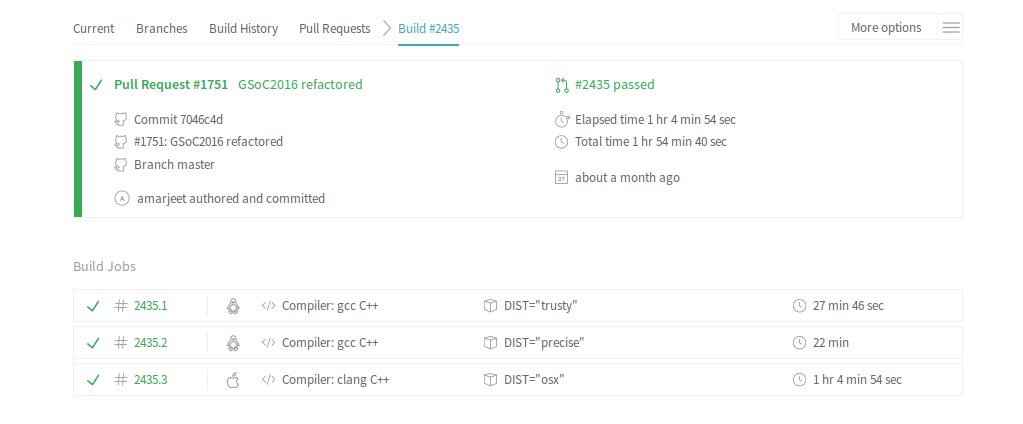
\includegraphics[width=\linewidth]{images/travis.png}
         \caption{Travis test summary for 3 different OS}
         \label{fig:travis}
     \end{figure}
     \begin{figure}
         \centering
         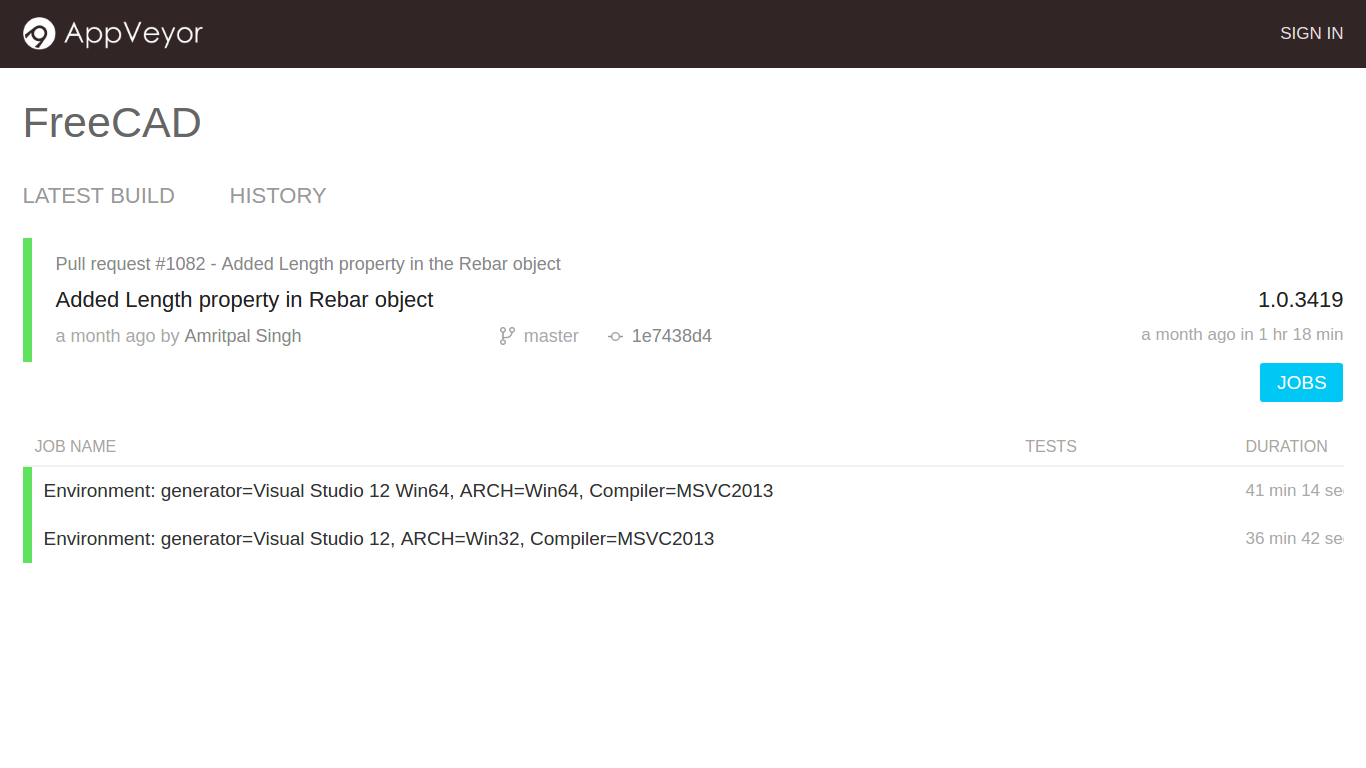
\includegraphics[width=\linewidth]{images/appveyor.png}
         \caption{AppVeyor test summary for Microsoft Windows virtual machine}
         \label{appveyor}
     \end{figure}
   
     \item \textbf{Regression Testing:} It is done by running the test cases developed for the OpenSCAD before the New changes are made to check whether new Changes doesn't produce abnormal behavior. Figure. \ref{regression}
   
     \begin{figure}
         \centering
         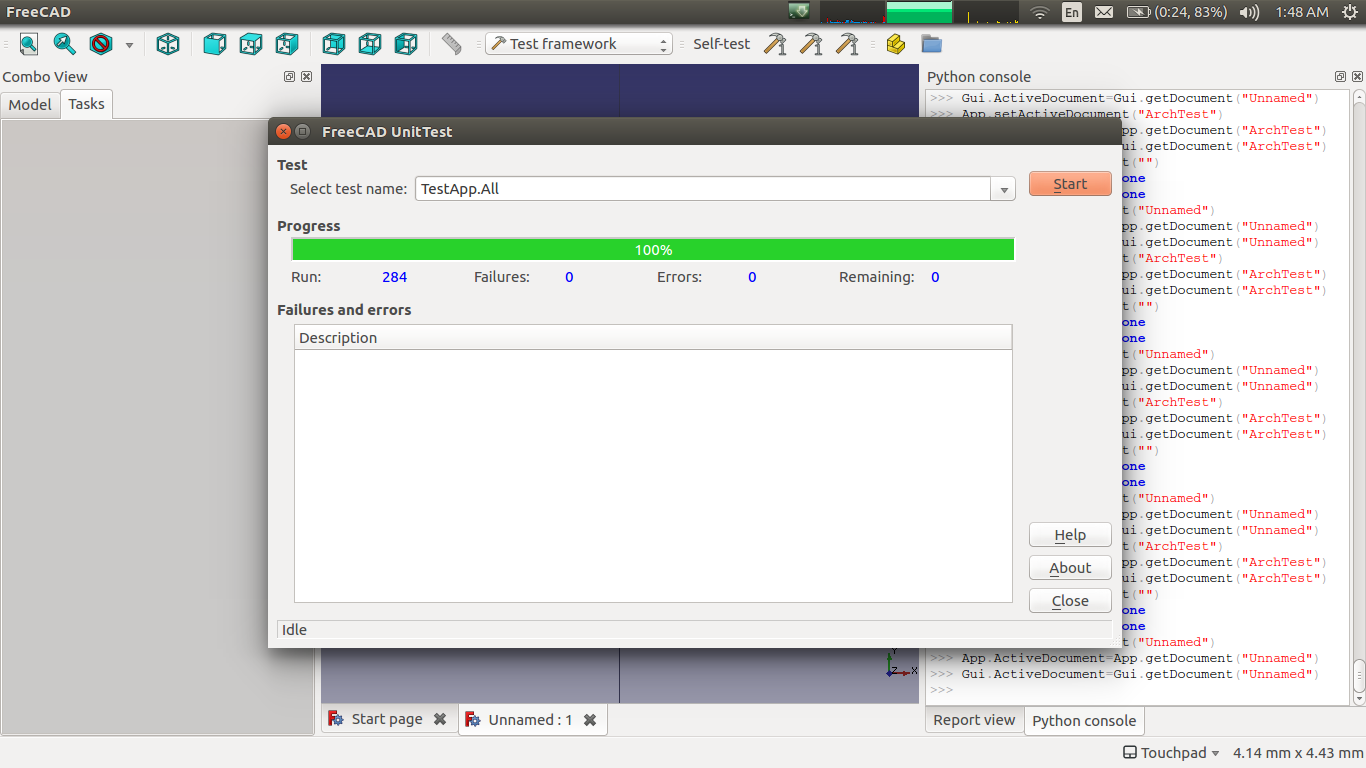
\includegraphics[width=\linewidth]{images/regression.png}
         \caption{Unit testing}
         \label{regression}
     \end{figure}
   
 \end{enumerate}


%\begin{sidewaystable}
%	\centering
%	\caption{Table to show various Tests}
%	 \begin{tabular}{ |c|c|c|c|c| }
%			\hline
%			\multicolumn{5}{|c|}{Test cases for customizer } \\
%			\hline
%			Sr. & Test Name & Test Description &No. of test Cases& Status \\ \hline
%			1 &customizertest\_description& Check if description syntax work& 24 &Pass\\ \hline
%			2 &customizertest\_parameter& Check if parameter syntax work& 33 &Pass\\ \hline
%			3 &customizertest\_allmodulescomment& Check iteraction of new syntax with modules & 39 &Pass\\ \hline
%			4 &customizertest\_allfunctionscomment & Check iteraction of new syntax with functionas&33 &Pass\\ \hline
%			5 &customizertest\_allexpressionscomment&Check iteraction of new syntax with expressions& 37&Pass\\ \hline
%			6 &customizertest\_group&  Check if group syntax work&16 & Pass\\ \hline
%			7 &customizertest-first\_setofparameter& Check if Json is read correctly& 1& Pass\\ \hline
%			8 &customizertest-wrong\_setofparameter&Check if Json is read correctly for wrong syntax& 1&Pass\\ \hline
%			9 &customizertest-incomplete\_setofparameter& Check if Json is read correctly for incomplete parameters& 1& Pass\\ \hline
%			10 &customizertest-imgset\_setofparameter&Check if Json is read correctly for imaginary set&1 & Pass\\ \hline	
%		\end{tabular}
%	\end{sidewaystable}
		
		
